\chapter{Theoretical background}
\label{ch:theoretical_background}

\section{Cloud-native and Web GIS}
\label{tb:cloud_native}
Cloud computing in this context refers to the infrastructure for delivering computing services including data storage, processing power, and applications over the internet, typically using the HTTP protocol. While "cloud" encompasses a broad range of meanings, \citet{nist_cloud_computing_2011} defines it as \emph{"Cloud computing is a model for enabling ubiquitous, convenient, on-demand network access to a shared pool of configurable computing resources (e.g., networks, servers, storage, applications, and services) that can be rapidly provisioned and released with minimal management effort or service provider interaction."}

The fundamental shift from desktop to cloud-based applications is reflected in the geospatial domain as well. For example, Google Maps Platform \citep{google_maps_platform} is widely used as a mapping application, with various features such as map delivery, navigation, and search provided as web services. Users do not need to download complete map datasets to their local machines.

In this research, the terms "Web GIS" and "cloud-based GIS" are used interchangeably to refer to geospatial technologies delivered through cloud technologies or provided over networks, in contrast to traditional desktop GIS applications that operate on local machines with locally stored data. This encompasses any GIS system that uses web technology to communicate between a server and a client, as defined by \citet{esri_webgis}, but emphasises the network-based delivery model that distinguishes it from standalone desktop applications. Throughout this research, "web" and "cloud" imply essentially the same meaning—systems that deliver geospatial services over networks rather than through local desktop applications.

\subsection{Advantages of Web GIS}
\label{tb:advantages_of_webgis}

\citet{esri_webgis} lists the advantages of Web GIS as follows:

\begin{itemize}
  \item \textbf{Global reach}: Web GIS applications can be accessed worldwide from computers or mobile devices, with HTTP protocol support enabling broad accessibility through organisational firewalls.
  \item \textbf{Scalability for multiple users}: Unlike desktop GIS limited to single users, web GIS can simultaneously support dozens or hundreds of users, requiring higher performance and scalability.
  \item \textbf{Cross-platform compatibility}: Web browsers (Internet Explorer, Firefox, Safari, Chrome) largely comply with HTML and JavaScript standards, enabling Web GIS to support different operating systems including Windows, Linux, and Mac OS.
  \item \textbf{Diverse applications}: Web GIS serves a broader audience beyond GIS professionals, supporting diverse applications such as mapping, photo tagging, location services, and various public-facing geospatial services.
\end{itemize}

\subsection{Challenges of Web GIS}
\label{tb:challenges_of_webgis}

Web GIS faces several significant challenges that distinguish it from traditional desktop GIS applications. Network latency and bandwidth limitations represent primary constraints. While local disk access in desktop applications can achieve high-speed read and write operations, Web GIS must transfer data over networks \citep{alesheikh_2002}. Loading 1GB of map data from a local machine versus downloading it over a network demonstrates this performance gap. This necessitates subsetting or streaming strategies where clients fetch only the data subsets they require. Traditional data formats such as GeoJSON, Shapefile, and WKT do not inherently support these selective access patterns.

Another challenge is multi-user scalability. Desktop GIS typically serves a single user, whereas Web GIS may serve hundreds or thousands of users simultaneously. To provide stable service, Web GIS must be scalable and robust under high concurrent load \citep{esri_webgis}.

\subsection{Strategies for Web GIS}
\label{tb:strategies_for_webgis}

To address Web GIS challenges while leveraging its advantages, several strategies are commonly employed:
\begin{itemize}
  \item \textbf{Tiling and partitioning}: Large datasets are divided into small, manageable tiles or chunks. Tile Map Service (TMS) exemplifies this approach by dividing maps into square tiles for each zoom level. As users zoom in or out, new tiles are loaded and displayed, with clients loading only necessary tiles. Figure \ref{fig:tms} shows an example of TMS, a standard for tiling geospatial data \citep{tms}. This technique requires either pre-generated tiled data or dynamic tile generation by servers like GeoServer \citep{geoserver}. Both raster and vector data are commonly tiled. This approach is not limited to 2D geospatial data; it is also used for 3D city model data. For instance, 3DBAG divides entire countries into tiles for selective download \citep{3dbag} and PLATEAU publishes tiled datasets as open data \citep{plateau}.

  \item \textbf{Spatial indexing}: Spatial indexing techniques index geospatial data by spatial properties. R-trees \citep{guttman_1984}, quadtrees \citep{finkel_1974}, and KD-trees \citep{bentley_1975} are commonly used indexing structures. These indices enable clients to quickly locate data within specified extents, find nearest neighbours, or perform other spatial queries. This technique requires pre-built spatial indices that must be updated when data changes.

  \item \textbf{Data simplification and Level of Detail}: Also known as generalisation, this reduces geospatial data complexity for visualisation, especially at smaller scales. This technique is often combined with tiling and partitioning. For example, Cesium 3D Tiles \citep{3d_tiles} implements level-of-detail systems where higher zoom levels load more detailed data. GDAL's Mapbox Vector Tile driver also supports geometry simplification for smaller scales \citep{gdal_mvt}.

  \item \textbf{Binary encoding and compression}: This technique reduces geospatial data size, resulting in faster download and display times. While compression reduces file size, it requires client-side decompression, creating a trade-off between file size and decompression time. For example, glTF 2.0 \citep{gltf_2_0}, used internally by Cesium 3D Tiles, supports Draco compression \citep{draco}. GeoParquet \citep{geoparquet} also supports various compression algorithms.
\end{itemize}

\begin{figure}[ht]
  \centering
  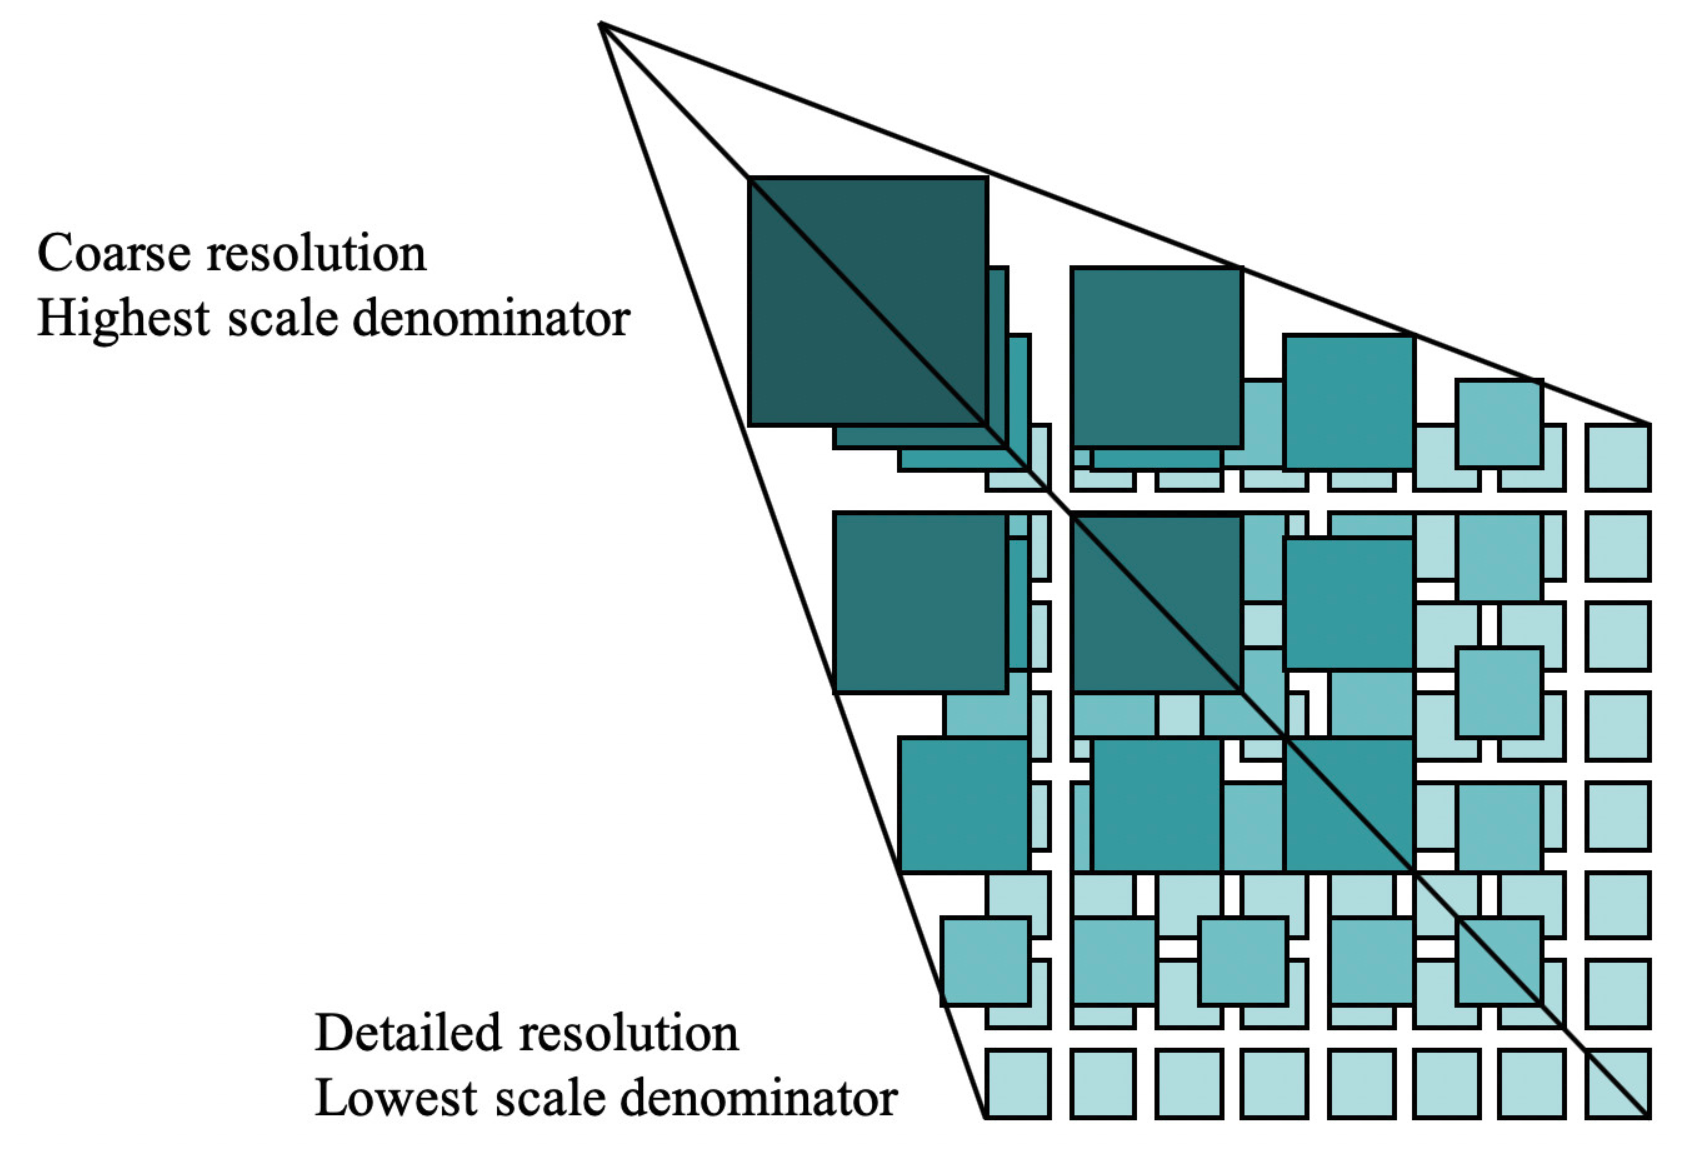
\includegraphics[width=0.7\textwidth]{figs/related_work_theoretical_bg/tms.png}
  \caption{Tile Map Service (TMS) standard for tiling geospatial data, derived from \citet{tms}}
  \label{fig:tms}
\end{figure}

When incorporating these strategies, the optimisation approaches that enable on-demand access to geospatial data are collectively referred to as \emph{cloud-optimised} formats \citep{cloud-optimised-formats}. The properties and related work of these cloud-optimised geospatial formats are discussed in detail in \autoref{rw:cloud_optimised_formats}.

\section{Binary file}
\label{tb:binary_file}
Binary file represents a fundamental approach to data storage that uses sequences of bits rather than human-readable text. Unlike plain text files that consist of characters interpreted through common character sets like ASCII, binary files store data in a format optimised for machine processing \citep{binary_file}.

Binary encoding offers several key advantages: superior storage efficiency through data compression and faster program execution. Binary files are commonly used for images, audio, executable programs, and compressed data.
However, binary encoding presents notable challenges. Binary files are not human-readable, making debugging, correction, or modification complex without specialised tools. Many binary systems are proprietary and platform-specific, creating portability issues and potential long-term accessibility problems. The Unix philosophy advocates for plain text storage when practical, emphasising that text serves as a universal interface enabling efficient program interoperability \citep{binary_file}.

In geospatial domains, prominent examples of text-based formats include GeoJSON \citep{geojson} and Geography Markup Language (GML) \citep{gml} as text representations for general geospatial data. For 3D city model data specifically, CityGML \citep{CityGML} and CityJSON \citep{cityjson} (including its streaming variant CityJSONSeq \citep{ledoux_2024}) represent the primary text-based standards. Conversely, binary geospatial formats include GeoPackage \citep{geopackage} and GeoTIFF \citep{geotiff}. Notably, no widely adopted standard binary formats currently exist for 3D city model data, representing a gap that this research aims to address.

\section{WebAssembly}
\label{tb:webassembly}
WebAssembly (WASM) is a low-level assembly-like language with a compact binary format that enables near-native performance execution in modern web browsers \citep{WebAssembly}. Standardised by the W3C \citep{WebAssemblyCoreSpecification1, WebAssemblyCoreSpecification2}, WebAssembly provides a compilation target for languages such as C/C++, C\#, and Rust, allowing code written in these languages to run efficiently on the web platform.

WebAssembly is designed to complement and run alongside JavaScript rather than replace it. Through the WebAssembly JavaScript APIs, developers can load WebAssembly modules into JavaScript applications and share functionality between the two environments \citep{WebAssembly}. This interoperability enables developers to leverage WebAssembly's performance characteristics for computationally intensive tasks while maintaining JavaScript's expressiveness and flexibility for application logic and user interface development.

A key advantage of WebAssembly is its ability to enable code reuse across platforms. Developers can compile existing codebases written in languages like C/C++, Rust, and C\# for browser deployment, eliminating the need to rewrite performance-critical components in JavaScript.

In this research, WebAssembly enables the compilation of Rust libraries for 3D city model processing to run with near-native performance in web browsers. This approach bridges the performance gap between desktop and web-based geospatial applications while maintaining the accessibility and cross-platform benefits of web deployment.

\section{Row-based and column-based data storage}
\label{tb:row_based_column_based_data_storage}

Data storage systems can be broadly categorised into two fundamental approaches: row-based and column-based storage. Row-based storage stores consecutive rows of a table sequentially, while column-based storage stores consecutive columns of a table sequentially \citep{clickhouse_column}.

To illustrate this distinction, consider the following example table:

\begin{verbatim}
id, city, country
1, Tokyo, Japan
2, London, UK
3, Amsterdam, Netherlands
\end{verbatim}

Row-based storage organises the data sequentially by rows:

\begin{verbatim}
1, Tokyo, Japan, 2, London, UK, 3, Amsterdam, Netherlands
\end{verbatim}

Column-based storage organises the data sequentially by columns:

\begin{verbatim}
1, 2, 3, Tokyo, London, Amsterdam, Japan, UK, Netherlands
\end{verbatim}

These different storage approaches exhibit distinct performance characteristics depending on the query patterns. Row-based approaches perform well for single-row searches, such as querying the record for Amsterdam. Conversely, column-based approaches excel at analytical queries that involve aggregating or filtering columns \citep{clickhouse_column}.

\citet{abadi_2008} provides a comprehensive comparison of column-stores versus row-stores, highlighting that column-based storage offers advantages in terms of storage efficiency and query performance for analytical workloads, while row-based storage is more suitable for Online Transaction Processing (OLTP) systems that require frequent lookups and updates.

In the context of geospatial data, column-based storage is particularly well-suited for analytical queries such as calculating the average height of buildings in a city or filtering buildings by construction year. However, row-based storage remains preferable for frequently updated datasets or transactional systems where individual records are accessed and modified regularly.
\section{CPU Caches}
\label{tb:cache}
Modern computing systems face a fundamental challenge to software performance due to the disparity between the speed of Central Processing Units (CPUs) and the latency of main memory. CPUs operate at clock speeds that far exceed the access speeds of dynamic random-access memory (DRAM), which typically serves as main memory. Consequently, the CPU frequently idles while waiting for data from the slower memory subsystem. To mitigate this performance bottleneck, CPU caches were developed. These caches utilise a small amount of very fast Static RAM (SRAM) to store temporary copies of data and instructions that are likely to be used again soon \citep{drepper_2007}.

The effectiveness of CPU caches hinges on two fundamental principles of program behaviour: temporal locality and spatial locality. Temporal locality refers to the tendency of a program to access data that has been recently accessed again in the near future. Spatial locality refers to the tendency of a program to access data that is located nearby in memory to previously accessed data. In other words, small chunks of data that have been accessed recently or are located nearby in memory are likely to be accessed again soon. Modern processors employ multiple levels of caches to maximise the effectiveness of these principles. This hierarchy typically consists of L1, L2, L3 caches, and main memory. The lower levels of the cache hierarchy are faster and smaller, while the higher levels are slower and larger \citep{drepper_2007}.

Data is not loaded into caches byte by byte. Instead, it is loaded in blocks called cache lines, typically 64 bytes in size. This design reduces the number of separate memory transactions and effectively amortises the substantial latency involved in accessing main memory \citep{drepper_2007}.

The performance of a cache is fundamentally determined by its hit rate. A cache hit occurs when the requested data is found within the cache, resulting in very fast access. In contrast, a cache miss occurs when the requested data is not found within the cache, necessitating a much slower retrieval from a higher-level cache or, in the worst case, main memory \citep{abayomi_2020}.

Understanding these aspects of cache behaviour is crucial when designing binary data formats, as cache-friendly data layouts can significantly improve application performance.

\section{Serialisation and Deserialisation}
\label{tb:serialisation_deserialisation}
Before discussing the specific techniques used in the FlatCityBuf format, it is important to understand the general principles of serialisation and deserialisation.

The terminology for data conversion processes varies across different programming ecosystems. Terms such as serialisation, pickling, marshalling, and flattening are often used interchangeably, though with subtle differences depending on the context. \citet{cpp_serialization} describes it from an object-oriented perspective as converting objects in memory (in a data structure) to a storable or transmittable format on disk. \citet{py_serialization} refers to this process as "pickling" in the Python ecosystem. For clarity in this thesis, we adopt the definition provided by \citet{viotti_2022}:

\begin{quote}
  "Serialisation is the process of translating a data structure into a bit-string (a sequence of bits) for storage or transmission purposes."
\end{quote}

Deserialisation is the reverse process of serialisation, where the bit-string is converted back into the original data structure (in memory).

\section{Zero-copy}
\label{tb:zero_copy}
Zero-copy is a technique used to avoid copying data from one memory location to another. The term "Zero-copy" is used in many contexts of computer science, \citet{song2012performance}  and \citet{brose_2008_zerocopy} provide a detailed explanation of the concept.

In conventional I/O operations, data typically traverses multiple memory regions, each requiring a separate copy operation:

\begin{itemize}
  \item Data is copied from storage devices into kernel buffer cache
  \item From kernel buffer, data is copied to user-space application buffers
  \item For network transmission, data may be copied again to network buffers
\end{itemize}

This multi-stage copying introduces significant overhead, particularly for large datasets or high-throughput applications. Each copy operation consumes CPU cycles, memory bandwidth, and increases latency \citep{song2012performance}. For applications working with large 3D city models, this overhead can substantially degrade performance.

\todo{Todo: improve here}
Zero-copy approaches optimise this data path by eliminating unnecessary copy operations. While "zero-copy" as a term suggests complete elimination of copying, in practice, different techniques achieve varying degrees of copy reduction:

\begin{itemize}
  \item \textbf{Memory-mapped \ac{io}}: Maps files directly into process address space, allowing direct access without explicit read/write operations
  \item \textbf{Direct \ac{io}}: Bypasses the kernel buffer cache for specific workloads
  \item \textbf{Scatter-gather \ac{io}}: Reads data directly into discontiguous memory regions
  \item \textbf{Shared memory}: Provides common address space for inter-process communication
  \item \textbf{In-place parsing}: Processes data structures without creating intermediate copies
\end{itemize}
\todo{ravi's comment "so this is in-place parsing, which also enables memory mapping? Are some other of the above terms also relevant? Clarify exactly how Flatbuffers relates to what you explain above."}

Modern serialisation formats like FlatBuffers implement zero-copy through carefully designed memory layouts that allow direct access to serialised data without requiring a separate deserialisation step. This approach is particularly valuable for geospatial applications that routinely handle large datasets.
\section{Endianness}
\label{tb:endianness}
Endianness (or "byte-order") refers to the order in which bytes are stored in memory when representing multi-byte values. The terminology was introduced by \citet{danny_cohen_1981}.

In computing, endianness becomes significant when multi-byte data types (such as 16-bit integers or 32-bit floats) must be stored in memory or transmitted across networks. There are two primary byte ordering systems:

\begin{itemize}
  \item \textbf{Little-endian}: Stores the least significant byte at the lowest memory address, followed by increasingly significant bytes. This is the ordering used by Intel processors that dominate desktop and server computing. For example, the 32-bit integer \texttt{0x12345678} would be stored in memory as 4 bytes: \texttt{0x78}, \texttt{0x56}, \texttt{0x34}, \texttt{0x12}.

  \item \textbf{Big-endian}: Stores the most significant byte at the lowest memory address. This approach is often called ``network byte order'' because Internet protocols typically require data to be transmitted in big-endian format. For example, the same 32-bit integer \texttt{0x12345678} would be stored as \texttt{0x12}, \texttt{0x34}, \texttt{0x56}, \texttt{0x78}.
\end{itemize}

A useful analogy is date notation: little-endian resembles the European date format (31 December 2050), while big-endian resembles the ISO format (2050-12-31), with the most significant part (year) first \citep{endianness_mdn}.

\section{Binary Search}
\label{tb:binary_search}

Binary search is a fundamental algorithm for finding elements in a sorted array. The classic implementation follows a simple approach: compare the search key with the middle element of the array, then recursively search the left or right half depending on the comparison result \citep{binary_search}.

The time complexity of binary search is logarithmic—the height of the implicit binary search tree is $\log_2(n)$ for an array of size $n$. While this is theoretically efficient, the actual performance suffers when implemented on modern hardware due to memory access patterns. Each comparison requires the processor to fetch a new element, potentially causing a cache miss (cache miss is explained in \autoref{tb:cache}). In the worst case, the number of memory read operations will be proportional to the height of the tree, with each read potentially requiring access to a different cache line or disk block \citep{binary_search}.

This inefficiency is particularly problematic when binary search is implemented on external memory or over HTTP, where each access incurs significant latency. The sorted array representation with binary search does not take advantage of CPU cache locality, as consecutive comparisons frequently access distant memory locations.

\subsection{Eytzinger Layout}
\label{tb:eytzinger_layout}

While preserving the same algorithmic idea as binary search, the Eytzinger layout (also known as a complete binary tree layout or level-order layout) rearranges the array elements to match the access pattern of a binary search \citep{binary_search}. Instead of storing elements in sorted order, it places them in the order they would be visited during a level-order traversal of a complete binary tree.

This layout significantly improves memory access patterns. When the array is accessed in the sequence of a binary search operation, adjacent accesses often refer to elements that are in the same or adjacent cache lines. This layout also proves beneficial for managing data fetched over networks, as consecutive elements accessed during binary search are more likely to be retrieved in the same HTTP range request, thereby reducing the number of network roundtrips and overall latency. This spatial locality enables effective hardware prefetching, allowing the CPU to anticipate and load required data before it is explicitly accessed, thus reducing latency \citep{binary_search}.

\autoref{fig:eytzinger_layout} shows how the layout appears when applied to binary search. \autoref{fig:eytzinger_layout2} shows that the algorithm starts from the first element and then jumps to either $2k$ or $2k+1$ depending on the comparison result. The heatmap represents the expected frequency of comparisons for search (the closer to the top, the more frequent the comparison).

\begin{figure}[ht]
  \centering
  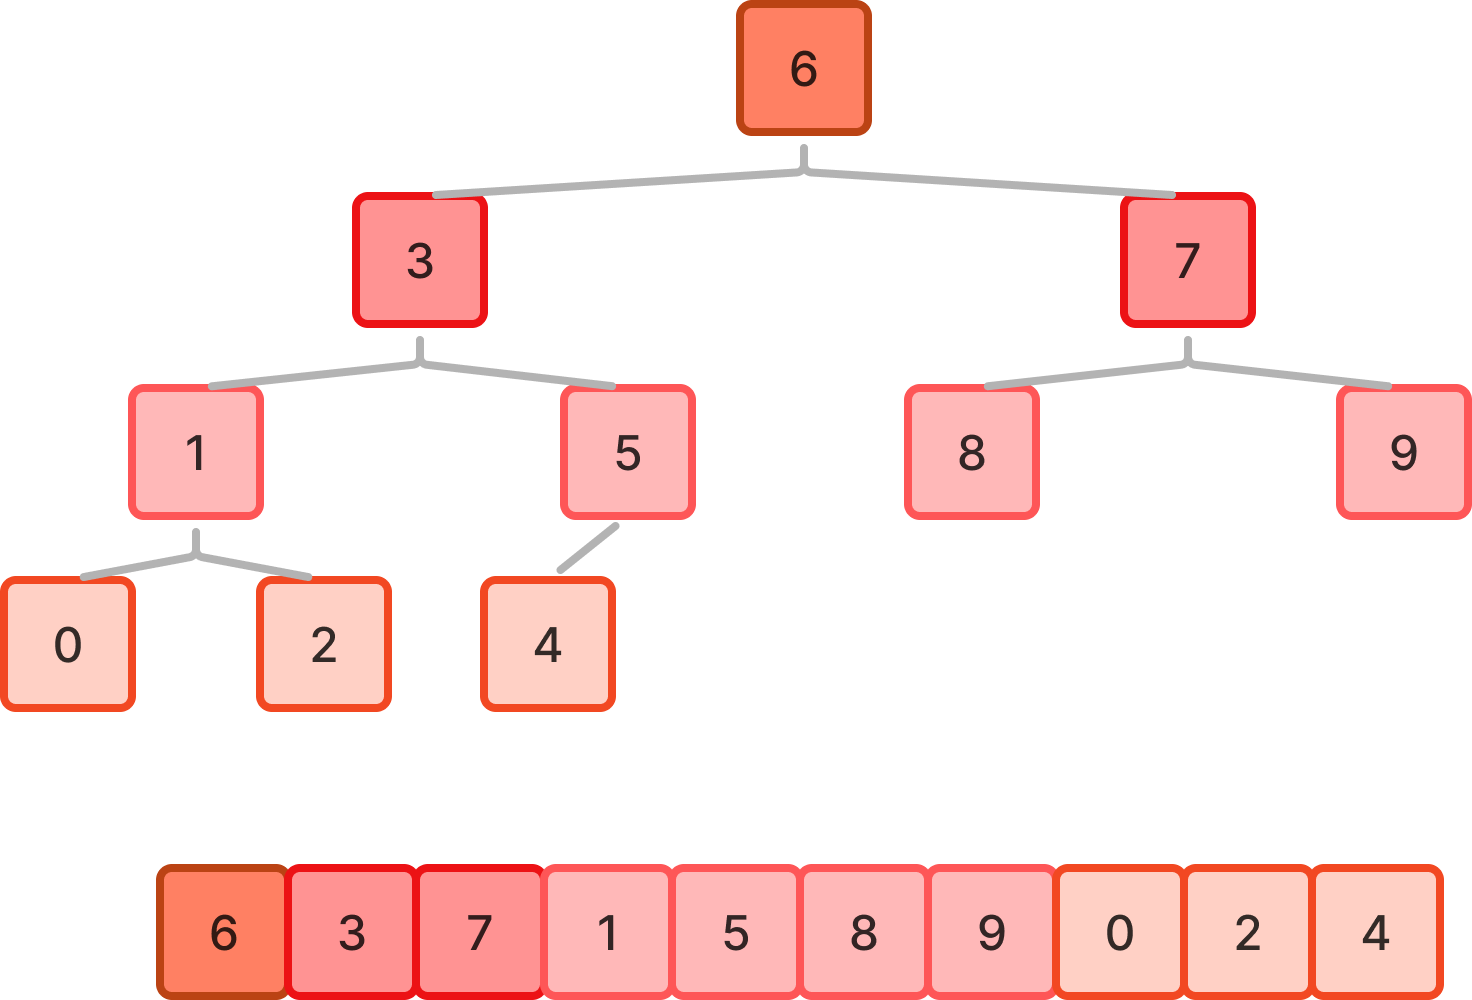
\includegraphics[width=0.5\textwidth]{figs/related_work_theoretical_bg/eytzinger_layout.png}
  \caption{Eytzinger layout as conceptual representation as tree and actual data layout (modified from \citet{binary_search})}
  \label{fig:eytzinger_layout}
\end{figure}
\begin{figure}[ht]
  \centering
  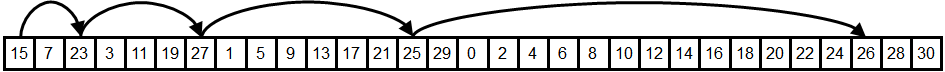
\includegraphics[width=0.5\textwidth]{figs/related_work_theoretical_bg/eytzinger_layout2.png}
  \caption{Binary search traversal pattern in Eytzinger layout (modified from \citet{binary_search})}
  \label{fig:eytzinger_layout2}
\end{figure}

\section{\texorpdfstring{\ac{s+tree}}{S+tree}}
\label{tb:static_btree}

\subsection{B-Tree/B+Tree Layout}
\label{tb:btree_layout}

While the Eytzinger layout improves cache utilisation for binary search, the number of memory read operations remains proportional to the height of the tree—$\log_2(n)$ for $n$ elements. This is still suboptimal for large datasets, especially when the access pattern involves disk \ac{io} or remote data access \citep{static_b_trees}.

B-Trees and their variants address this limitation by storing multiple keys in each node, effectively reducing the height of the tree. In a B-Tree of order $k$ (where each node can contain up to $k-1$ keys), the height of the tree is reduced from $\log_2(n)$ to $\log_k(n)$. This represents a reduction factor of $\log_k/\log_2 = \log_2(k)$ times compared to a binary search tree.

The key insight is that fetching a single node still takes roughly the same time regardless of whether it contains one key or multiple keys, as long as the entire node fits into a single memory block or disk page. By packing multiple keys into each node, B-Trees significantly reduce the number of disk or memory accesses required to locate an element.

B+Trees are a variant of B-Trees specifically optimised for range queries and sequential access patterns. In a B+Tree:
\begin{itemize}
  \item Internal nodes contain up to $B$ keys that serve as routing information, with each key associated with one of the $(B+1)$ pointers to child nodes. Each key at position $i$ represents the smallest key in the subtree pointed to by the $(i+1)$-th child pointer.
  \item Leaf nodes store the actual data with up to $B$ key-value pairs and include a pointer to the next leaf node, enabling efficient sequential traversal for range queries.
\end{itemize}

This linked structure of leaf nodes enables B+Trees to efficiently support range queries by traversing from one leaf to the next without needing to return to higher levels of the tree.

As the figure \ref{fig:btree_bplus_tree} shows, the B+Tree has pointers to the next leaf node, which enables efficient sequential traversal for range queries. On the other hand, the B+Tree has duplicate keys in the internal nodes, which is not the case for the B-Tree.

\begin{figure}[ht]
  \centering
  \begin{subfigure}[b]{0.45\textwidth}
    \centering
    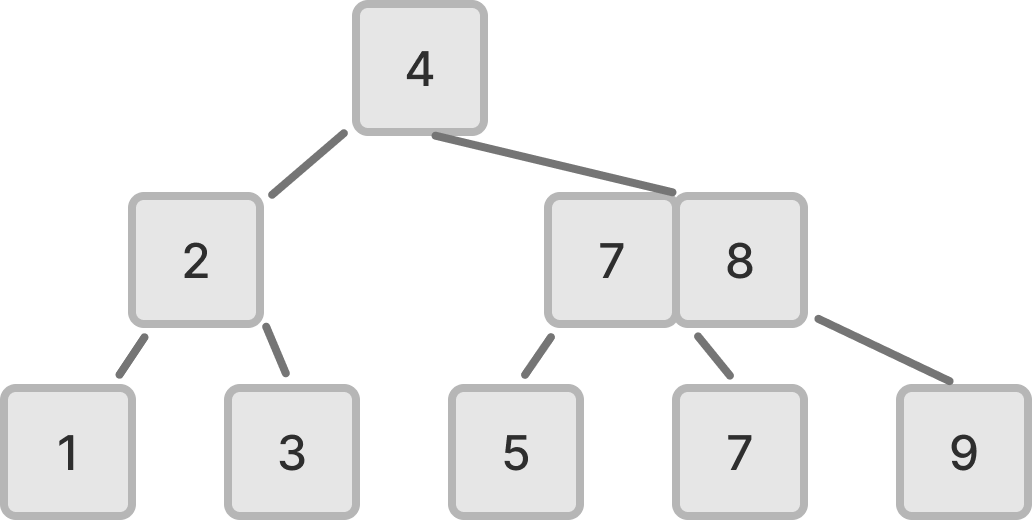
\includegraphics[width=\textwidth]{figs/related_work_theoretical_bg/btree.png}
    \caption{B-Tree (branching factor 3)}
    \label{fig:btree}
  \end{subfigure}
  \hfill
  \begin{subfigure}[b]{0.45\textwidth}
    \centering
    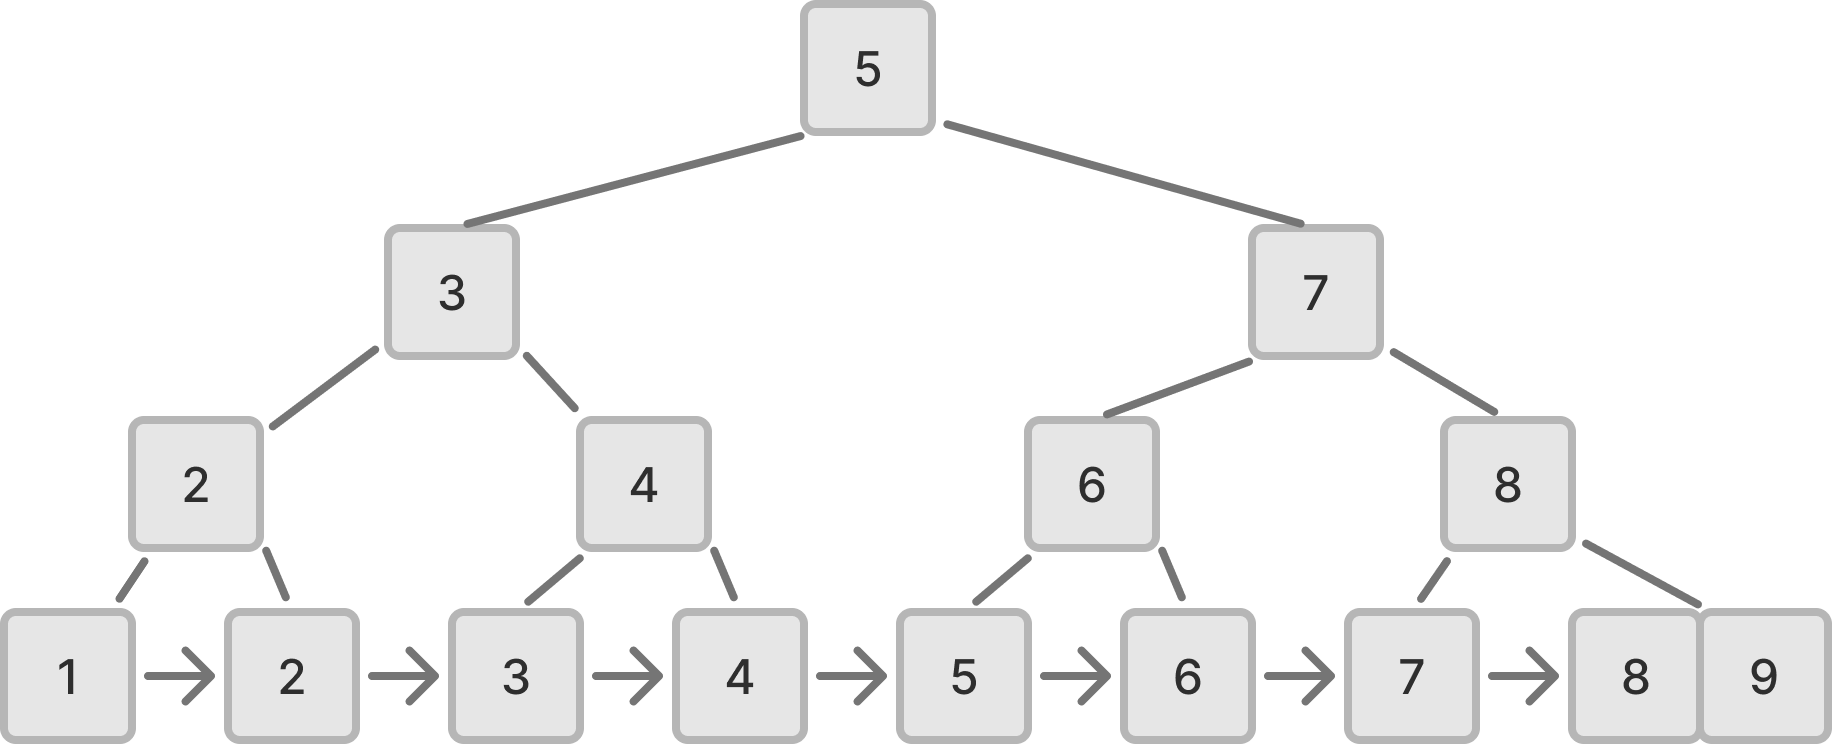
\includegraphics[width=\textwidth]{figs/related_work_theoretical_bg/bplus_tree.png}
    \caption{B+Tree (branching factor 3)}
    \label{fig:bplus_tree}
  \end{subfigure}
  \caption{B-Tree and B+Tree}
  \label{fig:btree_bplus_tree}
\end{figure}

\subsection{\texorpdfstring{\ac{s+tree}}{S+tree}}
\label{tb:stree}

The S+Tree (Static B+Tree), introduced by Algorithmica \citep{static_b_trees}, builds upon the B+Tree concept but is specifically designed for static datasets where the tree structure never changes after construction. Unlike traditional B+Trees that use explicit pointers between nodes, the S+Tree uses an implicit structure where child positions are calculated mathematically.
This is possible because:
\begin{itemize}
  \item The tree is constructed once and never modified (static)
  \item The number of elements is known in advance
  \item The tree can be maximally filled with no empty slots
  \item Child positions follow a predictable pattern based on the block size
\end{itemize}

For a \ac{s+tree} with block size $B$, a node with index $k$ has its children at indices calculated by a simple formula: $\text{child}_i(k) = k \cdot (B+1) + i + 1$ for $i \in [0, B]$ \citep{static_b_trees}. This eliminates the need to store and fetch explicit pointer values, further reducing memory usage and improving cache efficiency.

The S+Tree layout aligns with modern hardware characteristics where:
\begin{itemize}
  \item The latency of fetching a single byte is comparable to fetching an entire cache line (64 bytes)
  \item Disk and network I/O operations have high initial latency but relatively low marginal cost for additional bytes
  \item CPU cache lines typically hold multiple array elements (e.g., 16 integers in a 64-byte cache line)
\end{itemize}

By loading a block of $B$ elements at once and performing a local search within that block, S+Trees reduce the total number of cache misses or disk accesses to $\log_B(n)$ instead of $\log_2(n)$—a significant reduction for large datasets.

The S+Tree layout achieves up to 15× performance improvement over standard binary search implementations while requiring only 6-7\% additional memory \citep{static_b_trees}. This makes it particularly valuable for applications that perform frequent searches on large, relatively static datasets, especially when accessed over high-latency connections. For more detailed implementation strategies of S+Tree, \citet{koerkamp_2024} provides comprehensive explanations and practical considerations.